%%
%% This is file `sample-sigconf-authordraft.tex',
%% generated with the docstrip utility.
%%
%% The original source files were:
%%
%% samples.dtx  (with options: `all,proceedings,bibtex,authordraft')
%% 
%% IMPORTANT NOTICE:
%% 
%% For the copyright see the source file.
%% 
%% Any modified versions of this file must be renamed
%% with new filenames distinct from sample-sigconf-authordraft.tex.
%% 
%% For distribution of the original source see the terms
%% for copying and modification in the file samples.dtx.
%% 
%% This generated file may be distributed as long as the
%% original source files, as listed above, are part of the
%% same distribution. (The sources need not necessarily be
%% in the same archive or directory.)
%%
%%
%% Commands for TeXCount
%TC:macro \cite [option:text,text]
%TC:macro \citep [option:text,text]
%TC:macro \citet [option:text,text]
%TC:envir table 0 1
%TC:envir table* 0 1
%TC:envir tabular [ignore] word
%TC:envir displaymath 0 word
%TC:envir math 0 word
%TC:envir comment 0 0
%%
%% The first command in your LaTeX source must be the \documentclass
%% command.
%%
%% For submission and review of your manuscript please change the
%% command to \documentclass[manuscript, screen, review]{acmart}.
%%
%% When submitting camera ready or to TAPS, please change the command
%% to \documentclass[sigconf]{acmart} or whichever template is required
%% for your publication.
%%
%%
%\documentclass[acmsmall]{acmart}
\documentclass[sigconf]{acmart}
\usepackage{mathtools}
\usepackage{xspace} 
\usepackage{multirow}
%%
%% \BibTeX command to typeset BibTeX logo in the docs
\AtBeginDocument{%
  \providecommand\BibTeX{{%
    Bib\TeX}}}

%% Rights management information.  This information is sent to you
%% when you complete the rights form.  These commands have SAMPLE
%% values in them; it is your responsibility as an author to replace
%% the commands and values with those provided to you when you
%% complete the rights form.
\setcopyright{acmlicensed}
\copyrightyear{2025}
\acmYear{2025}
\acmJournal{TOG}

%% These commands are for a PROCEEDINGS abstract or paper.
% \acmConference[Conference acronym 'XX]{Make sure to enter the correct
%   conference title from your rights confirmation email}{June 03--05,
%   2025}{Woodstock, NY}
%%
%%  Uncomment \acmBooktitle if the title of the proceedings is different
%%  from ``Proceedings of ...''!
%%
%%\acmBooktitle{Woodstock '18: ACM Symposium on Neural Gaze Detection,
%%  June 03--05, 2018, Woodstock, NY}
%\acmISBN{978-1-4503-XXXX-X/2025/06}


%%
%% Submission ID.
%% Use this when submitting an article to a sponsored event. You'll
%% receive a unique submission ID from the organizers
%% of the event, and this ID should be used as the parameter to this command.
\acmSubmissionID{papers\_353s1}

%%
%% For managing citations, it is recommended to use bibliography
%% files in BibTeX format.
%%
%% You can then either use BibTeX with the ACM-Reference-Format style,
%% or BibLaTeX with the acmnumeric or acmauthoryear sytles, that include
%% support for advanced citation of software artefact from the
%% biblatex-software package, also separately available on CTAN.
%%
%% Look at the sample-*-biblatex.tex files for templates showcasing
%% the biblatex styles.
%%

%%
%% The majority of ACM publications use numbered citations and
%% references.  The command \citestyle{authoryear} switches to the
%% "author year" style.
%%
%% If you are preparing content for an event
%% sponsored by ACM SIGGRAPH, you must use the "author year" style of
%% citations and references.
%% Uncommenting
%% the next command will enable that style.
\citestyle{acmauthoryear}


%%
%% end of the preamble, start of the body of the document source.
\begin{document}
%%
%% The "title" command has an optional parameter,
%% allowing the author to define a "short title" to be used in page headers.
\title{Leaf-alias: real-time importance sampling of dynamic emissive textures}

%%
%% The "author" command and its associated commands are used to define
%% the authors and their affiliations.
%% Of note is the shared affiliation of the first two authors, and the
%% "authornote" and "authornotemark" commands
%% used to denote shared contribution to the research.

\author{Jose Aguerre}
\affiliation{%
  \institution{Universidad de la República}
  \city{Montevideo}
  \country{Uruguay}}
\email{jpaguerre@fing.edu.uy}

\graphicspath{{images/}}
%%
%% By default, the full list of authors will be used in the page
%% headers. Often, this list is too long, and will overlap
%% other information printed in the page headers. This command allows
%% the author to define a more concise list
%% of authors' names for this purpose.
% \renewcommand{\shortauthors}{Trovato et al.}
\newcommand{\FLIP}{\protect\reflectbox{F}LIP\xspace}
%%
%% The abstract is a short summary of the work to be presented in the
%% article.
\begin{abstract}
We present a method for fast importance sampling HDR textured lights that allows real-time video-driven lighting. 
Our method partitions a light’s texture into a budgeted, variance driven quadtree and builds an alias table over the resulting leaves, avoiding the cost of a dense per-frame CDF while still capturing
the texture’s overall energy distribution. We present two variants: one that reuses the hierarchical structures already present in the metadata of modern codec video streams, and another that builds a budgeted GPU-friendly quadtree to fit the entire sampling structure in L1 cache.
Compared to the dense 2D CDF-inversion baseline, at a matched real-time frame-time budget our implemented technique reduces
RMSE by 9–53\% depending on scene, letting the saved sampling cost be reinvested in additional light samples.
It also reduces memory consumption and transfers by several orders of magnitude when compared to state of the art samplers.

\end{abstract}

%%
%% The code below is generated by the tool at http://dl.acm.org/ccs.cfm.
%% Please copy and paste the code instead of the example below.
%%
\begin{CCSXML}
<ccs2012>
   <concept>
       <concept_id>10010147.10010371.10010372.10010376</concept_id>
       <concept_desc>Computing methodologies~Reflectance modeling</concept_desc>
       <concept_significance>500</concept_significance>
       </concept>
 </ccs2012>
\end{CCSXML}

\ccsdesc[500]{Computing methodologies~Reflectance modeling}

%%
%% Keywords. The author(s) should pick words that accurately describe
%% the work being presented. Separate the keywords with commas.
\keywords{These are the keywords}
%% A "teaser" image appears between the author and affiliation
%% information and the body of the document, and typically spans the
%% page.

% \begin{teaserfigure}
%   \centering
%   \begin{tabular}{@{}c@{}c@{}c@{}c@{}}
%     \setlength{\fboxsep}{2pt}  % space between image and border
%     \setlength{\fboxrule}{1pt} % border thickness
%     \includegraphics[width=0.24\textwidth, trim=250 0 250 0, clip]{teaser/horse.png} &
%     \includegraphics[width=0.24\textwidth, trim=250 0 250 0, clip]{teaser/micrograin.png} &
%     \includegraphics[width=0.24\textwidth, trim=250 0 250 0, clip]{teaser/sheen.png} &
%     \includegraphics[width=0.24\textwidth, trim=250 0 250 0, clip]{teaser/rocks.png} \\[0pt]
%     \framebox{\includegraphics[width=0.15\textwidth]{micro_samples/ggx_style.pdf}} &
%     \framebox{\includegraphics[width=0.15\textwidth, trim=0 90 0 90, clip]{micro_samples/3.pdf}} &
%     \framebox{\includegraphics[width=0.15\textwidth, trim=0 0 0 90, clip]{micro_samples/palitos.pdf}} &
%     \framebox{\includegraphics[width=0.15\textwidth]{micro_samples/2.pdf}} \\[0pt]
%     GGX Style heightfield &
%     Ellipsoidal micrograins &
%     Microfibers &
%     Random circle particles \\
%     Specular bounces &
%     Specular bounces & 
%     Glossy bounces &
%     Lambertian bounces
%   \end{tabular}
%   \caption{Microgeometries designed and rendered with our tool.}
%   \label{fig:teaser}
% \end{teaserfigure}

\begin{teaserfigure}
  \centering
  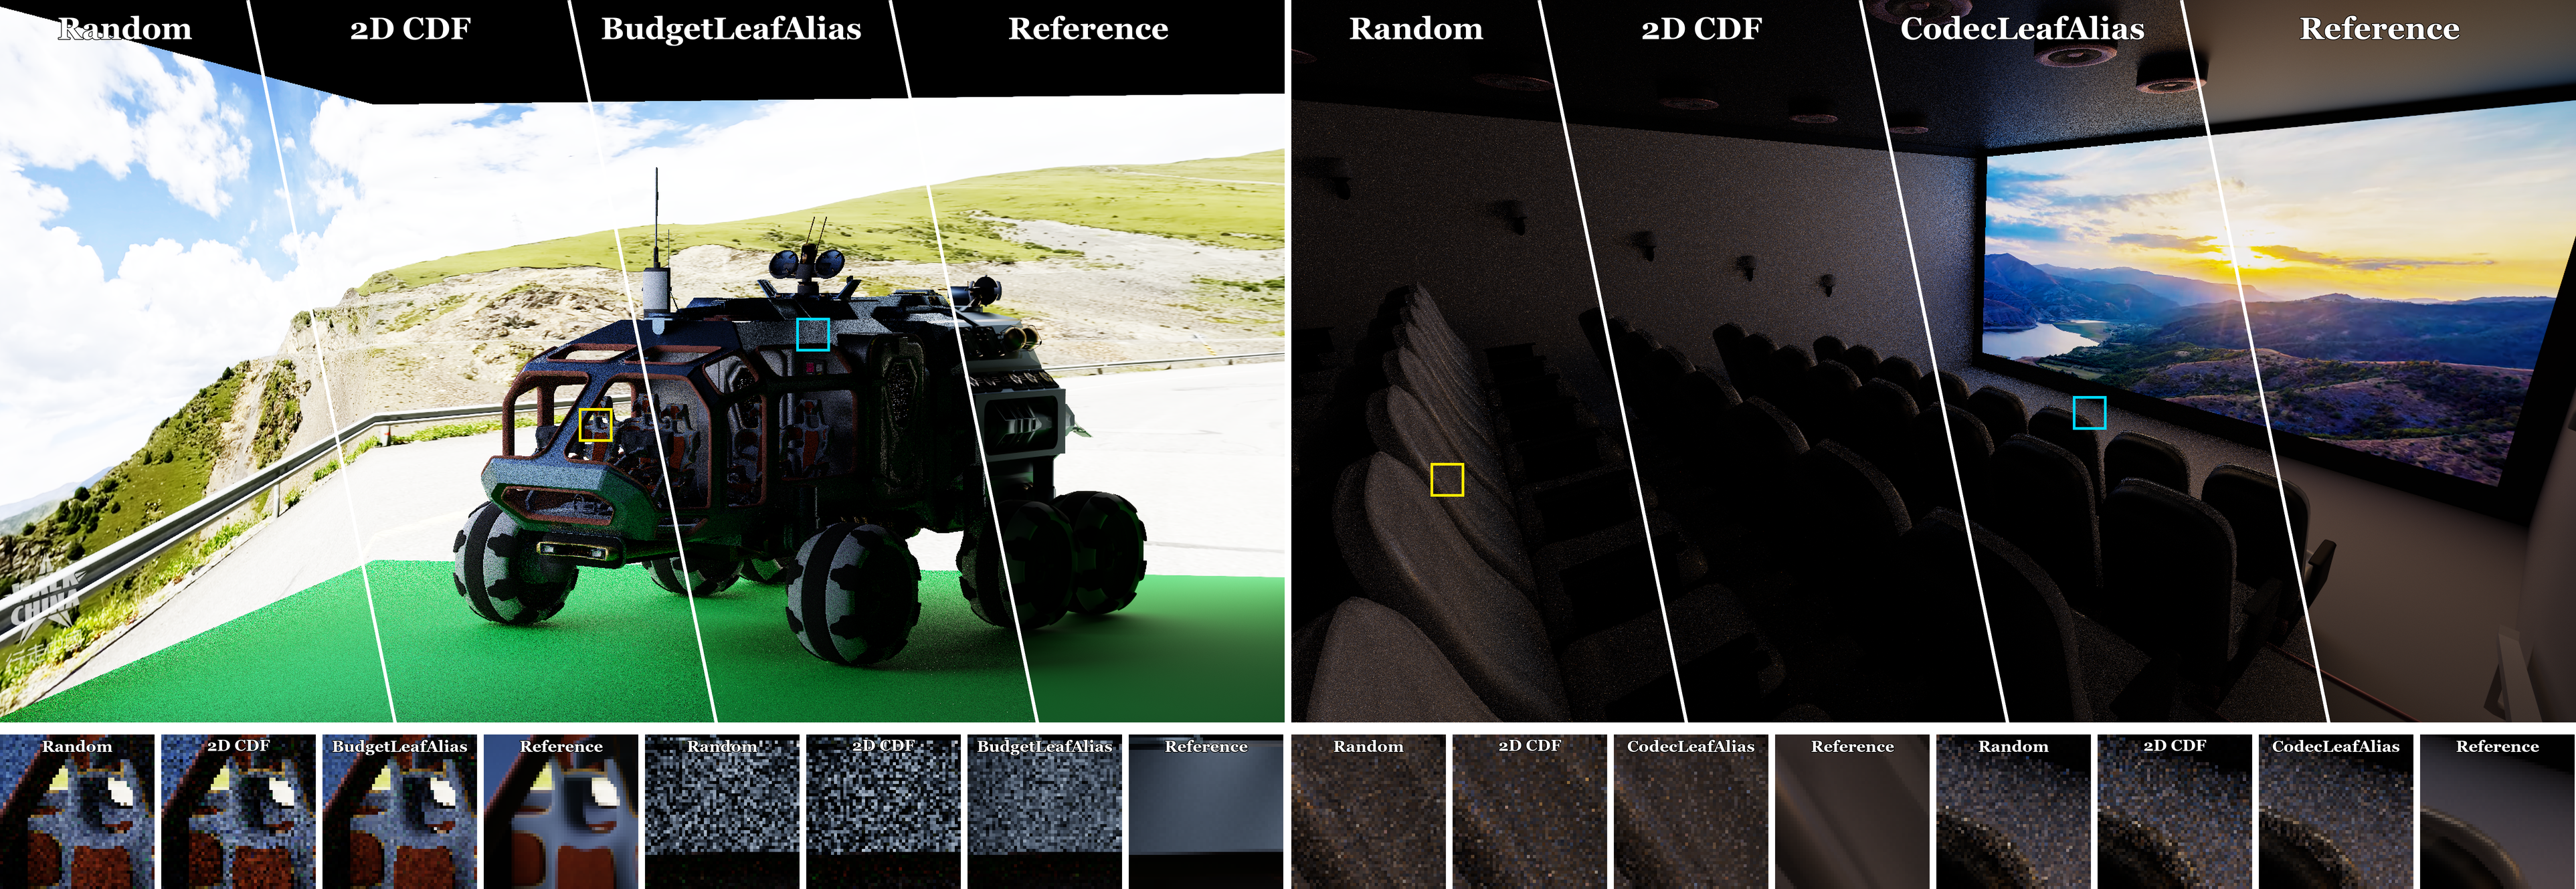
\includegraphics[width=1\textwidth]{teaser.png}
  \caption{Two scenes lit by a single dynamic, video-driven emissive texture, rendered with our leaf-alias importance sampler. (Left) The Rover scene — a virtual-production LED wall displaying a looping road/mountain video panorama that lights the vehicle directly, sampled here with BudgetLeafAlias. (Right) The Cinema scene — a theater lit only by the animated sunset footage playing on its own screen, sampled with CodecLeafAlias. Each panel compares, left to right: Random sampling, 2D CDF inversion, our technique, and a converged reference, all at their calibrated real-time budgets ($\approx$33 ms).}
  \label{fig:teaser}
\end{teaserfigure}



%%
%% This command processes the author and affiliation and title
%% information and builds the first part of the formatted document.
\maketitle

\section{Introduction}

Importance sampling of emissive textures is essential for efficient image-based lighting, and increasingly critical in production workflows where video is used directly as a dynamic light source in virtual production and VFX. A single emissive texture lets a renderer reproduce the directional detail of a real environment, far beyond what analytic lights can approximate. Traditionally this texture has been static, captured once and reused for an entire sequence. Increasingly, though, it is video: LED-wall virtual production, AR/VR object insertion, and video-based environment lighting all require illumination that changes every frame, not a single fixed capture. 

Traditional texture light sampling techniques are designed for static images. They rely on the offline building of large sampling structures that are reused for rendering each frame as long as the image doesn't change. The most common example of such strategy is how rendering and ray tracing toolboxes deal with HDR environment maps. The state-of-the-art approach is to build a two-dimensional piecewise constant distribution from the texture’s luminance: a marginal CDF over rows and a per-row conditional CDF. The sampler is then inverted via binary search at sample time, which is expensive for large textures. A more recent and well-adopted approach is to generate a mipmap-style hierarchical importance map \cite{}. At sample time, a hierarchical descent through a mip pyramid
of the texture is performed, recursively choosing one of four children at each level in proportion to their summed weight. This technique is also expensive and requires several iterations per sample, although it is more GPU friendly because the number of iterations is always the same for each sample, unlike in the binary search.  Moreover, the mipmap can be fastly constructed using the existing dedicated hardware on modern GPUs. Both techniques require at least $O(N)$ memory for the sampler, with $N$ being the number of pixels.

Another less used but known technique for sampling emissive textures is the Alias method \cite{}. This technique draws from an arbitrary discrete distribution in $O(1)$ time after an $O(N)$ one-time build, at the cost of losing the CDF's implicit spatial coherence: two adjacent table buckets can alias to two arbitrary, unrelated locations in the original distribution. This fact is known to disrupt the stratification or disrepancy-reduction of the input point set. It also requires $O(N)$ memory to store the correlation between every pixel. The process for building the Alias table, despite being $O(N)$, is difficult to optimize for real-time construction \cite{}. 

We present a new sampling method that is fast to build (under 1 millisecond for 4k HDR images), produces a sampler that is tiny, and is $O(1)$ to sample without disrupting the stratification of the Quasi Monte Carlo input. The core idea is to reuse the variance-driven image partition that is already present in modern video codecs, which already compute hierarchical spatial partitions that adapt to local signal variance \cite{uhrina2024performance}. These structures implicitly encode the spatial distribution
of luminance and high-frequency content (see Fig. \ref{fig:quadtree}). We also propose a variant that builds the partition tree on a budgeted number of leaves, using a  Greedy/best-first tree-structured resource allocation \cite{MINASNY2007383,Zhou2024}. Both techniques show consistent quality gains when rendering video light textures in real-time (33 milliseconds per frame), since they allow executing more texture samples without  introducing stratification error.

\begin{figure}[htbp!]
  \centering
  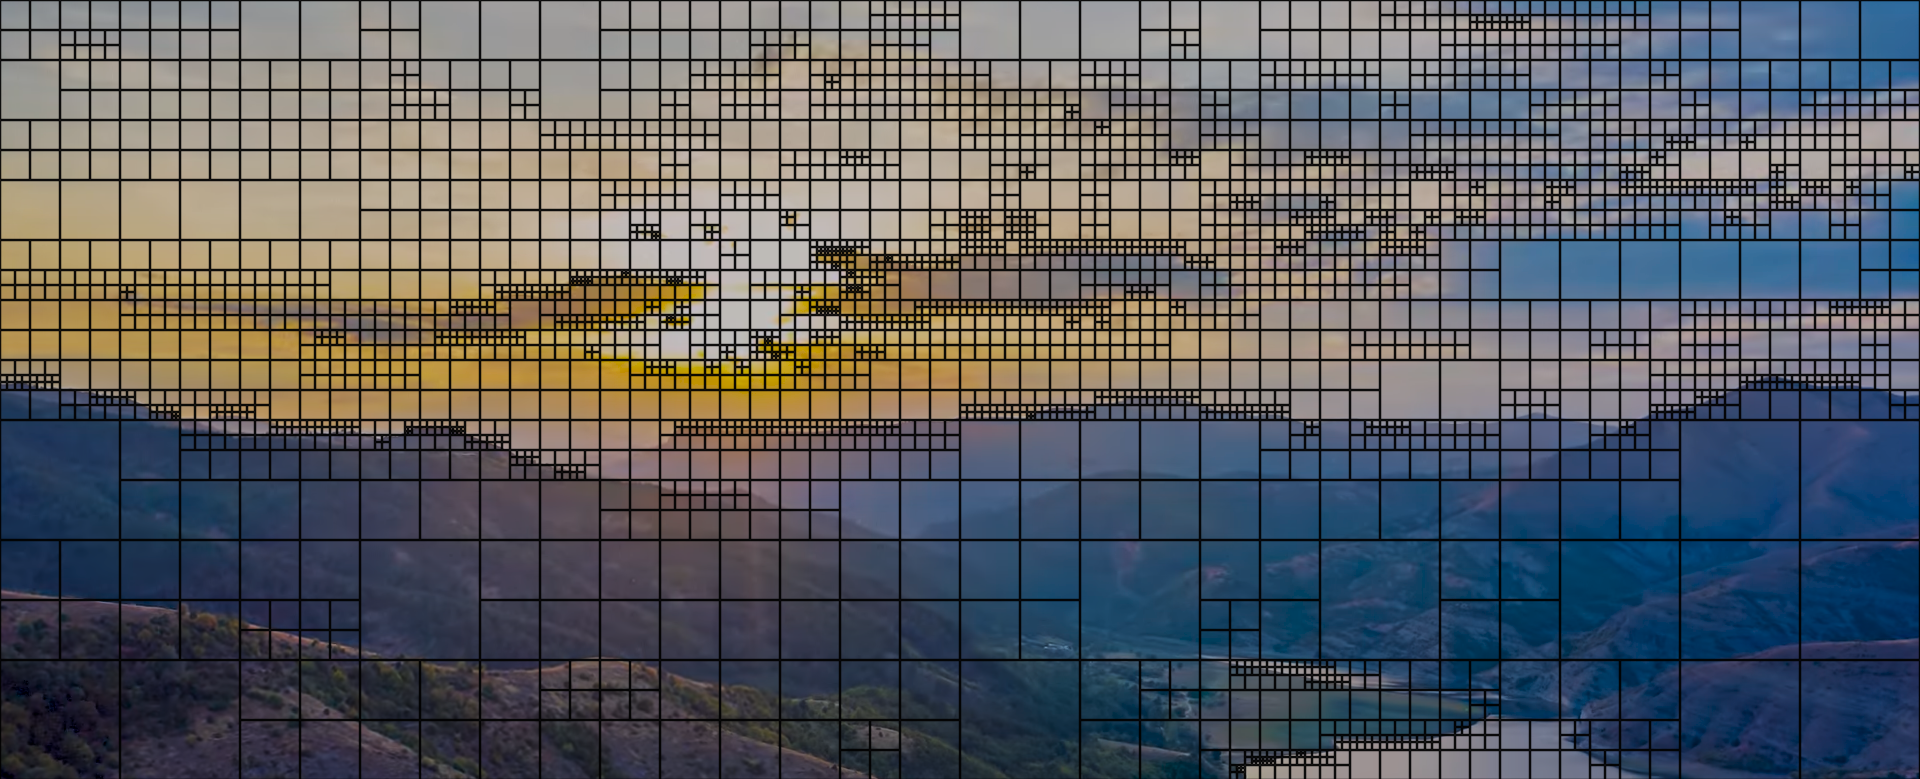
\includegraphics[width=\linewidth]{quadtree.png}
  \caption{An example of a variance-driven quadtree built by the VP9 video codec. High variance zones are refined into a dense mesh of
  small cells.}
  \label{fig:quadtree}
\end{figure}

\section{Previous works}\label{sec:prev}
Importance sampling of emissive textures is a well-studied problem in the graphics literature in the context of image-based lighting. Most of the works focus on pre-processing the images to allow for exact or near-exact sampling without introducing bias \cite{lawrence2005adaptive}. Several methods choose to simplify the textured light into a set of point or area lights ~\cite{agarwal2003structured}, allowing for real-time sampling and faster convergance but at the cost of more error in the solution.  Cline et al. \cite{cline2009tabular} compare several tabular inversion methods, noting the computational order of building each sampler structure and sampling each point. They analyze the 2D CDF inversion via binary search and the per-pixel Alias method, where they flag the disruption of the stratification of the input point set. Per-pixel Alias's raster-flattened table produces a real, measurable periodic banding pattern (Figure~\ref{fig:spectrum}) that becomes clear in
the sample set's power spectrum. We show that our LeafAlias method overcomes those issues because the partition structure helps with stratification. 

\begin{figure}[htbp!]
  \centering
  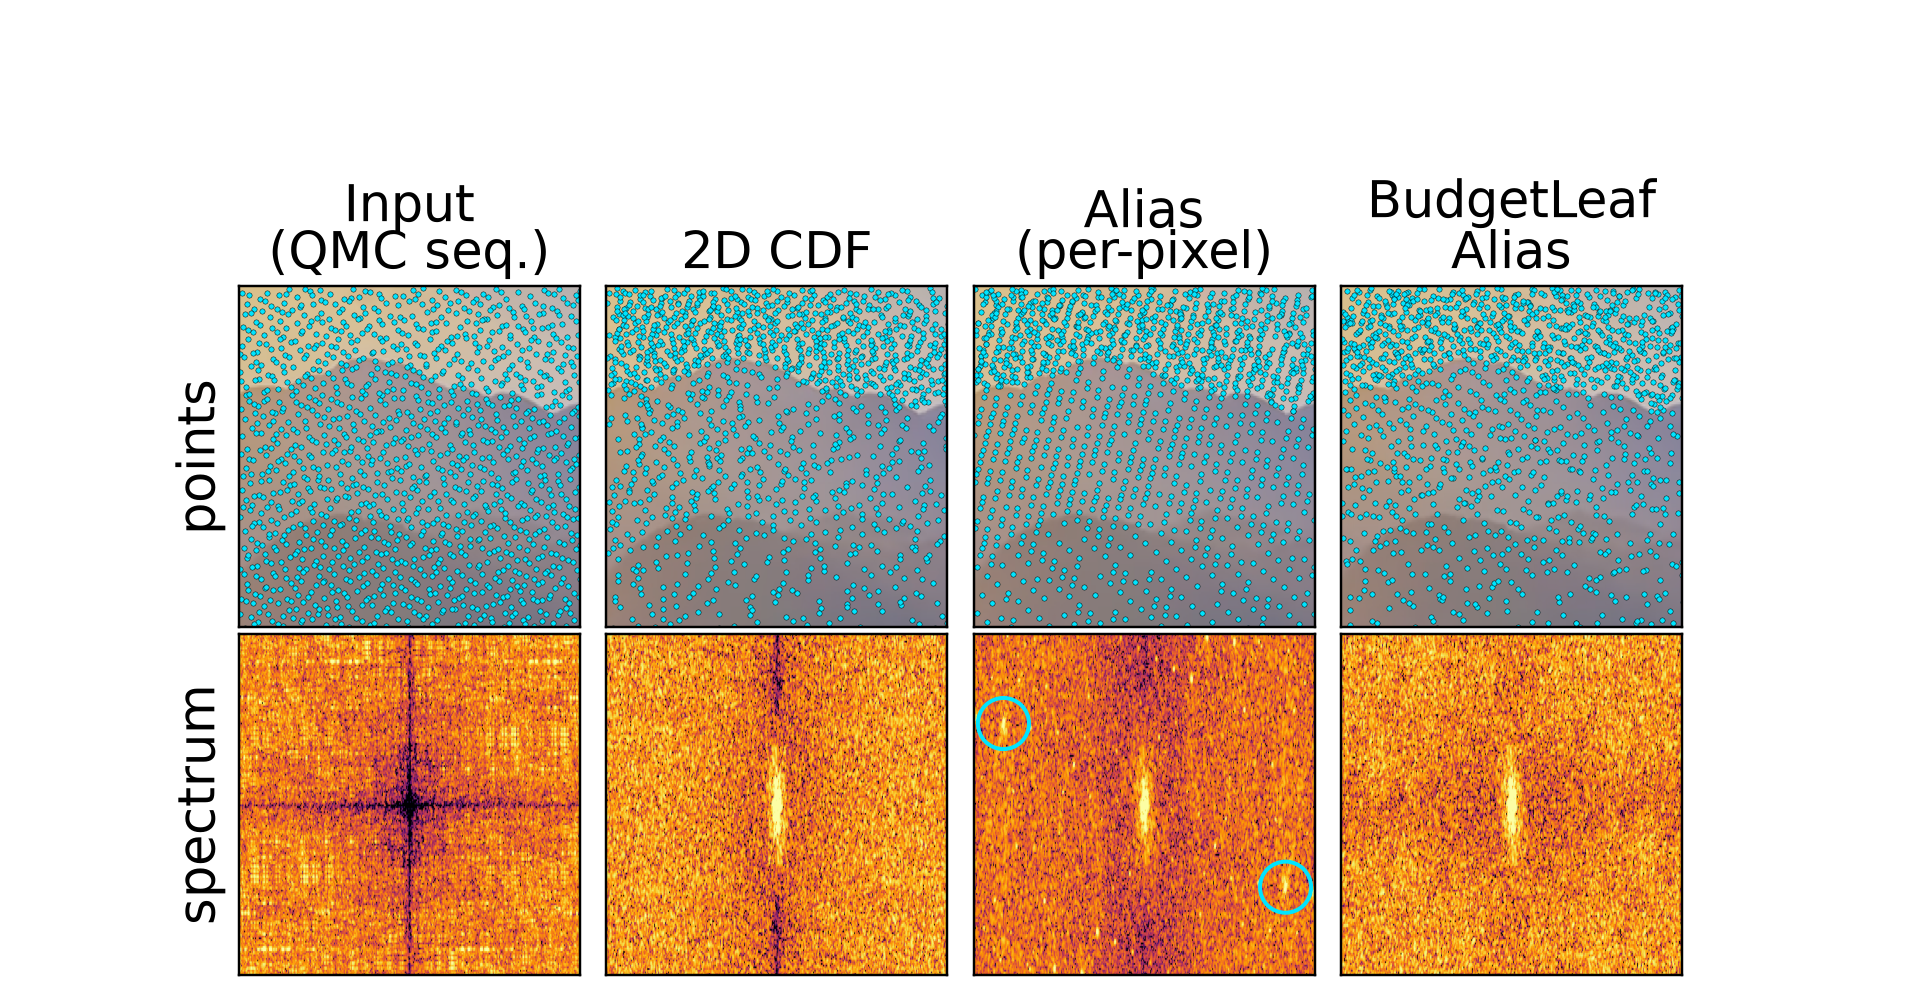
\includegraphics[width=\linewidth]{fig_spectrum_paper_color.png}
  \caption{2D power spectrum of samples from 2D CDF inversion, plain per-pixel alias, and
  our LeafAlias, from the same Halton input. Per-pixel alias shows a sharp,
  isolated off-axis peak (flatness 0.270, peak/median 16{,}113) -- a periodic banding
  artifact from its flat array index resonating with the input sequence's base-2 digit
  structure. Both CDF inversion and ours stay close to the input's own clean spectrum.}
  \label{fig:spectrum}
\end{figure}

Despite being $O(1)$ to sample, the per-pixel Alias method is heavy in memory consumption and in the construction of the tables via Vose's technique. 
Nevertheless, the Alias method is widely used in mesh lights sampling: geometry with thousands of emissive triangles. Moreau et al.~\cite{moreau2019dynamic} maintain a light-sampling BVH incrementally across frames for thousands of moving lights.
Bitterli et al.'s ReSTIR~\cite{bitterli2020spatiotemporal} resamples across spatial and
temporal neighbors to pick among many dynamic lights at a fraction of the cost of resampling
from scratch. Conty Estevez and Kulla~\cite{contykulla2018adaptive} adaptively split a light
tree per shading point rather than committing to one fixed cut. At that scale of thousands of triangles, a plain alias table over per-triangle flux is common practice
and cheap to rebuild every frame.

Regarding the optimization of the sampling structures, 
Ergun et al.~\cite{ergun2012realtime} split an environment map into a kd-tree via the greedy partition strategy, to a predefined block count, then fit the sorted leaf probabilities with a closed-form curve for direct inversion. They report gains in memory compression, higher speed and accuracy than CDF inversion at matched performance for static environment maps. One disadvantage of using kd-trees is that evaluating the pdf of the map direction when sampled from BRDF in MIS requires traversing the tree.  
 Lambers~\cite{lambers2022parameterization} proposes a fixed-grid sampler and notes that replacing the grid with a variance-driven quadtree might improve their results. Rodrigues et al.~\cite{rodriguez2023nenv} train a neural normalizing flow that allows both sampling and evaluating the pdf, showing considerable performance gains at the cost of pre-training the structure for the static map. Wu~\cite{wu2025efficient} also preprocess the map by dividing the emissive and non-emissive parts into separate structures. 

The previously described techniques focus mainly in preprocessing static images to improve sampling efficiency, but not dynamic maps. Some previous works address video-driven lighting: Havran et al.~\cite{havran2005interactive} and Iorns and Rhee~\cite{iorns2015realtime} both light scenes from captured video environment maps, but neither targets real-time per-frame
resampling of the video itself as the importance distribution. Lu et al.~\cite{lu2013realtime} rebuild a tabulated per-cube-face CDF in real-time, noting it as an expensive part of the process.  Kronander et al~\cite{kronander2014real} rely on temporal sample reuse to improve convergance of video-based lighting. 

Attempts to make the per-frame rebuild itself cheaper on a GPU point the same direction: Morrical and Zellmann~\cite{morrical2021inverse} accelerate 2D CDF
inversion with ray-tracing hardware at high construction cost and non-trivial implementation
complexity. Lehmann et al.~\cite{lehmann2021weighted} study GPU-specific weighted sampling and alias-table construction directly. 



Current open-source renderers mostly rely on dense CDF or mipmapped samplers. {Falcor}~\cite{falcorsoftware} uses a hierarchical mip-pyramid importance map over the environment texture's luminance and, separately,
the triangle-scale alias table for mesh lights. {Mitsuba 3}~\cite{nimierdavid2019mitsuba2} builds a {Hierarchical2D} warp over
the environment map -- the same mip-pyramid family as Falcor's. {pbrt-v4}~\cite{pharr2023pbrt}
uses a dense CDF distribution, inverted via binary search. {Blender Cycles}~\cite{cyclessoftware} builds the same
kind of dense marginal/conditional CDF over a downsampled background map. Every one of the four either assumes the environment
texture is built once and reused.

\section{Method}\label{sec:method}
This is the method
\subsection{Codec-leaf-alias}
\subsection{Budget-leaf-alias}

\section{Results} \label{sec:results}
These are the results 

\section{Conclusions and future work} \label{sec:conclusions}
These are the conclusions
\bibliographystyle{ACM-Reference-Format}
\bibliography{sample-base}

\end{document}